\documentclass[12pt]{article}

\usepackage{mathtools}
\usepackage{algorithm}
\usepackage{algpseudocode}
\usepackage[margin=1in]{geometry}
\usepackage{amsmath,amsthm,amssymb}
\usepackage{graphicx}
\usepackage{tikz}
\usetikzlibrary{calc}

\DeclarePairedDelimiter\ceil{\lceil}{\rceil}
\DeclarePairedDelimiter\abs{\lvert}{\rvert}%
\setlength\parindent{0pt}

\begin{document}

\pagestyle{myheadings}
\markboth{\hfill\hfill Team 5}{Team 5 \hfill\hfill}

\title{Simple Operating System\\Documentation}
\author{Tong Wu - z3417604\\Lewis Lee - z3415068}

\maketitle

\clearpage

\tableofcontents

\clearpage

\section{Assumptions \& Known Issues}
\begin{itemize}
\item Maximum processes name length is 32 characters long
\item Error checking with processes is not robust
\item Demand paging uses FIFO, not Second Chance algorithm. Not sure where to obtain the referenced bit for a frame.
\item Swapping does not work with multiple processes running, we start getting cap faults at random places.
\end{itemize}

\section{Clock Driver}
\subsection{Interface}
The clock driver is implemented using the EPIT1 and EPIT2 timers and implements the following functions;

\begin{itemize}
\item \textbf{int} start\_timer(\textbf{seL4\_CPtr} interrupt\_ep1, \textbf{seL4\_CPtr} interrupt\_ep2)\\
This is called to initialize both EPIT1 and EPIT2 timers. It takes in two \textbf{seL4\_CPtr}s and sets them as interrupt endpoints for EPIT1 and EPIT2 respectively. If the timers are already running (ie start\_timer had been called before), then they will be stopped and restarted. \textbf{CLOCK\_R\_OK} will be returned on success, otherwise \textbf{CLOCK\_R\_FAIL} will be returned.

\item \textbf{uint32\_t} register\_timer(\textbf{uint64\_t} delay, \textbf{timer\_callback\_t} callback, \textbf{void} *data)\\
This is called to set a timer which will expire after a given delay while calling a given callback function. If timers are not initialized, \textbf{CLOCK\_R\_UINT} will be returned, \textbf{CLOCK\_R\_FAIL} will be returned if the maximum number of timers is reached (this is currently 50, this can be changed in clock.h). \textbf{CLOCK\_R\_OK} will be returned on success.

\item \textbf{int} remove\_timer(\textbf{uint32\_t} id)\\
This is an internal function which when called, removes the timer from the priority queue.

\item \textbf{int} EPIT1\_interrupt(\textbf{void})\\
This function should normally be called when there is a timer interrupt for \textbf{EPIT1} (used for heartbeats). When called, it will update the current time and reset the underflow flag (so the timer will continue to interrupt). It then acknowledges the interrupt handler. If \textbf{EPIT1} is not initialized, \textbf{CLOCK\_R\_UINT} will be returned, otherwise \textbf{CLOCK\_R\_OK} will be returned.

\item \textbf{int} EPIT2\_interrupt(\textbf{void})\\
This function should normally be called when there is a timer interrupt for \textbf{EPIT2} (used for callback timers). When called, it will call the callback function for the current timer in queue, then removes the timer from queue using \textbf{remove\_timer()}. If \textbf{EPIT2} is not initialized, \textbf{CLOCK\_R\_UINT} will be returned, otherwise \textbf{CLOCK\_R\_OK} will be returned.

\item \textbf{timestamp\_t} time\_stamp(\textbf{void})\\
This function prints out the current time after \textbf{start\_timer()} was called. It checks the underflow flag in case it missed an interrupt and adds additional time if necessary. Then it adds the time elapsed since the last interrupt to the current time and returns the current time in microseconds (64-bit unsigned integer). If \textbf{EPIT1} is not initialized, \textbf{CLOCK\_R\_UINT} will be returned.

\item \textbf{int} stop\_timer(\textbf{void})\\
This function can be called to stop all current callback timers and to do a soft reset on both \textbf{EPIT1} and \textbf{EPIT2}. \textbf{CLOCK\_R\_UINT} will be returned if the timers are not initialized, otherwise \textbf{CLOCK\_R\_OK} will be returned.
\end{itemize}

\subsection{Configurables}
\begin{itemize}
\item\textbf{PRESCALAR\_EPIT1}: Controls the prescale value for EPIT1, currently set to 6.
\item\textbf{PRESCALAR\_EPIT2}: Controls the prescale value for EPIT2, Currently set to 66.
\item\textbf{TIMER\_TICK\_INTERVAL}: Controls the amount of timer ticks between each interrupt for EPIT1, currently set to 1100000.
\item\textbf{MAX\_TIMERS}: Controls the maximum amount of timers we can have registered at once, currently set to 50.
\end{itemize}
The current values for PRESCALAR\_EPIT1 and TIMER\_TICK\_INTERVAL means that we get interrupts at 10Hz (100ms intervals) and due to the large TIMER\_TICK\_INTERVAL, we can get up to micro second accuracy since we can determine time passed between heart beats by reading the counter values directly.

\subsection{Operation}
In SOS, the clock driver is initialized on boot before the entering the main syscall loop. The EPIT1 interrupt is used for the 100ms heart beat and EPIT2 is used for timers (used to implement sleep). 

\clearpage
\section{Frame Table}
\subsection{Interface}
\begin{itemize}
\item \textbf{int} frametable\_init(\textbf{void})\\
Initialises the frame table
\item \textbf{int} frame\_alloc(\textbf{seL4\_Word} *vaddr)\\
Maps a page to the vaddr given, returns a paddr
\item \textbf{int} frame\_free(\textbf{seL4\_Word} vaddr)\\
Frees the paddr given
\item \textbf{int} frametable\_add\_page\_cap(\textbf{seL4\_CPtr} cap, \textbf{seL4\_Word} sos\_vaddr)\\
Add a page cap to the corresponding frame of frametable
\item \textbf{int} frametable\_map\_app\_page(\textbf{pid\_t} pid, \textbf{seL4\_CPtr} cap, \textbf{seL4\_Word} sos\_vaddr, \textbf{seL4\_Word} app\_vaddr)\\
Maps an app allocated page
\item \textbf{seL4\_CPtr} frame\_get\_cap(\textbf{seL4\_Word} vaddr)\\
Returns the page cap associated with a frame
\end{itemize}
\subsection{Structure}
The frametable is simply an contiguous array of frames. The frametable itself resides at a fixed offset past DMA region.

Each frame contains the following data;
\begin{itemize}
\item \textbf{seL4\_CPtr} cptr
\item \textbf{seL4\_CPtr} page\_cptr
\item \textbf{seL4\_Word} app\_vaddr
\item \textbf{pid\_t} pid\\
The process that owns the frame
\item \textbf{int} next\_swap\_frame\\
The next frame in the swap queue for demand paging
\item \textbf{int} prev\_swap\_frame\\
The previous frame in the swap queue for demand paging
\item \textbf{int} swap\_send\_count
\item \textbf{int} spare
\end{itemize}
\subsection{Operation}
Our frametable keeps track of allocated frames (physical memory which has been retyped and mapped). It maps one to one in a region of virtual memory past the DMA region. It keeps track of which addrspace it belongs to (and related information) as well as caps for freeing and mapping memory.

\clearpage
\section{Page Table/Address Space}
\subsection{Interface}
\begin{itemize}
\item \textbf{struct addrspace} *addrspace\_create(\textbf{void})\\
Create a new address space with first page level initialized
\item \textbf{int} sos\_map\_page\_table(\textbf{struct addrspace} *as, \textbf{seL4\_Word} vaddr)\\
Maps a second level table into the given page directory (1st level)
\item \textbf{int} sos\_map\_page(\textbf{pid\_t} pid, \textbf{seL4\_Word} vaddr, \textbf{seL4\_ARM\_VMAttributes} attr, \textbf{int} swappable)\\
Map a physical address to a page
\item \textbf{int} sos\_define\_region(\textbf{struct addrspace} *as, \textbf{seL4\_CapRights} permissions, \textbf{int} start, \textbf{int} end)\\
Defines a usable region for the application
\item \textbf{int} check\_region(\textbf{struct addrspace} *as, \textbf{seL4\_Word} vaddr, \textbf{seL4\_CapRights} *permissions)\\
Check whether a region is valid and extract its permissions
\item \textbf{seL4\_CPtr} app\_vaddr\_frame\_cap(\textbf{struct addrspace} *as, \textbf{seL4\_Word} app\_vaddr)\\
Return the frame cap for the corresponding application virtual address
\item \textbf{seL4\_Word} get\_sos\_vaddr(\textbf{ addrspace} *as, \textbf{seL4\_Word} app\_vaddr)\\
Given an address space and application address, returns the corresponding sos virtual address
\item \textbf{void} set\_cur\_as(\textbf{struct addrspace} *as)\\
Set the cur\_as (a global variable identifying the address space of the last process that sent a syscall)
\item \textbf{uint32\_t} expand\_virtual\_heap(\textbf{uint32\_t} newbrk)\\
Expands the virtual heap for the application, used by sys\_brk
\item \textbf{void} addrspace\_destroy(\textbf{struct addrspace} *as)\\
Destroy the given address space
\item \textbf{int} sos\_map\_elf\_page(\textbf{struct addrspace} *as, \textbf{seL4\_Word} kvpage, \textbf{seL4\_Word} vpage)\\
sed for mapping elf pages, as kdst needs to be mapped.
\end{itemize}
\subsection{Structure}
\subsection{Operation}
Our two level pagetable keeps track of the relevant memory information related to a process. This includes things such as whether a page is in file or memory and where in memory it is located. There is also another table which keeps track of pagetable details (paddr and caps) so that items can be freed correctly. Each pagetable also keeps a region list in which applications can access memory when a page fault is triggered. 
The key function of addrspace is to map pages between our OS and applications.

\clearpage
\section{System Calls}
\subsection{Overview}
In the application side, the system call functions determines the SOS system call number and sends data through IPC Message Registers and blocks until a reply comes from SOS. For sending and receiving large amounts of data, the libsos sends a pointer to an empty array, which will get translated, page by page by SOS, and filled. When a reply is received, libsos will retrieve data from the message registers and for large data, SOS would have filled it in already.

When SOS receives a system call, it retrieves the system call number from message register 0 and uses it to index an array of function pointers pointing to the corresponding hand system call function. When SOS is finished handling the system call, it replies and the application will resume.
\subsection{Interface}
\subsubsection{Application System Calls}
\begin{itemize}
\item \textbf{fildes\_t} sos\_sys\_open(\textbf{const char} *path, \textbf{int} flags)\\
Opens console if path is "console" otherwise, tries to open the given path from the file system.
flags can be \textbf{O\_RDONLY}, \textbf{O\_WRONLY} or \textbf{O\_RDWR}
\item \textbf{int} sos\_sys\_close(\textbf{fildes\_t} file)\\
Closes the file given by the file handle
\item \textbf{int} sos\_sys\_read(\textbf{fildes\_t} file, \textbf{char} *buf, \textbf{size\_t} nbyte)\\
Reads the file given by the file handle, using the function pointer to the correct read function (eg. tty or nfs) defined when the file was opened. tries to read nbytes but can return with less than that amount.
\item \textbf{int} sos\_sys\_write(\textbf{fildes\_t} file, \textbf{const char} *buf, \textbf{size\_t} nbyte)\\
Write to the file given by the file handle, using the function pointer to the correct write function defined when the file was opened.
\item \textbf{int} sos\_getdirent(\textbf{int} pos, \textbf{char} *name, \textbf{size\_t} nbyte)\\
Get directory entry given by pos from nfs.
\item \textbf{int} sos\_stat(\textbf{const char} *path, \textbf{sos\_stat\_t} *buf)\\
Returns information about file "path".
\item \textbf{pid\_t} sos\_process\_create(\textbf{const char} *path)\\
Creates a new process running the executable "path".
\item \textbf{int} sos\_process\_delete(\textbf{pid\_t} pid)\\
Deletes the process given by "pid".
\item \textbf{pid\_t} sos\_my\_id(\textbf{void})\\
Returns the pid of the current process.
\item \textbf{int} sos\_process\_status(\textbf{sos\_process\_t} *processes, \textbf{unsigned} max)\\
Returns the status of currently running processes. Max specifies the maximum number of process statuses to return.
\item \textbf{pid\_t} sos\_process\_wait(\textbf{pid\_t} pid)\\
Waits for the process given by pid to finish before resuming. If pid is -1 then wait for anything to finish before resuming.
\item \textbf{int64\_t} sos\_sys\_time\_stamp(\textbf{void})\\
Returns the current time since boot in microseconds.
\item \textbf{void} sos\_sys\_usleep(\textbf{int} msec)\\
Waits for "msec" milliseconds before resuming.resuming
\item \textbf{long} sys\_brk(\textbf{va\_list} ap)\\
Increases the heap region to a new brk point determined by "ap".
\end{itemize}
\subsubsection{Internal Functions}
All handle syscall functions in SOS have void return type and take one argument, "mypid" (PID of the caller application extracted from the incoming badge). Functions are called by indexing an array of function pointers to the handle syscall function corresponding to the syscall number.

Currently implemented syscall numbers are;
\begin{enumerate}
\item SOS\_SYS\_OPEN
\item SOS\_SYS\_CLOSE
\item SOS\_SYS\_READ
\item SOS\_SYS\_WRITE
\item SOS\_SYS\_GETDIRENT
\item SOS\_SYS\_STAT
\item SOS\_SYS\_PROCESS\_CREATE
\item SOS\_SYS\_PROCESS\_DELETE
\item SOS\_SYS\_MYID
\item SOS\_SYS\_PROCESS\_STATUS
\item SOS\_SYS\_PROCESS\_WAIT
\item SOS\_SYS\_TIMESTAMP
\item SOS\_SYS\_USLEEP
\item SOS\_SYS\_BRK
\item SOS\_TTY\_OPEN
\item SOS\_TTY\_CLOSE
\item SOS\_TTY\_WRITE
\item SOS\_TTY\_READ
\item SOS\_SYS\_CREATE
\end{enumerate}

\subsection{Coroutines}
We use coroutines sparingly and it was only first introduced to handle demand paging. Prior to that all our system calls relies purely on blocking and replying to the application through the method provided by seL4.
For coroutines, we are using an open source library called "picoro". The reason we chose picoro is because it provides us with a minimal number of functions we need to use coroutines effectively and its code base is extremely small (less than 100 lines), thus easy to understand. Picoro provides the following functions;
\begin{itemize}
\item \textbf{coro} coroutine(\textbf{void} *fun(\textbf{void} *arg))\\
Create a new coroutine that executes the given function when resumed for the first time
\item \textbf{int} resumable(\textbf{coro} c)\\
Returns whether the coroutine is resumable
\item \textbf{void} *resume(\textbf{coro} c, \textbf{void} *arg)\\
Resumes the given coroutine
\item \textbf{void} *yield(\textbf{void} *arg)\\
Yield from the coroutine we are currently in
\end{itemize}

Picoro has been added as a library, "libpicoro" to our code and some slight modifications were made to the picoro code in order for correct operation with SOS.
Each coroutine has a stack of 16KB, used to store local variables when we switch coroutines.
Each process has its own coroutine, created during each system call.
\clearpage
\subsection{Operation}
Below is a diagram of how our system calls generally operate. Blue lines indicate flow within SOS, red lines within an application and black lines indicate IPC. The large rounded rectangles are coroutines and everything inside belongs to that coroutine. Smaller rounded rectangles indicate a coroutine operation. 
\begin{figure}[htbp]
\centering
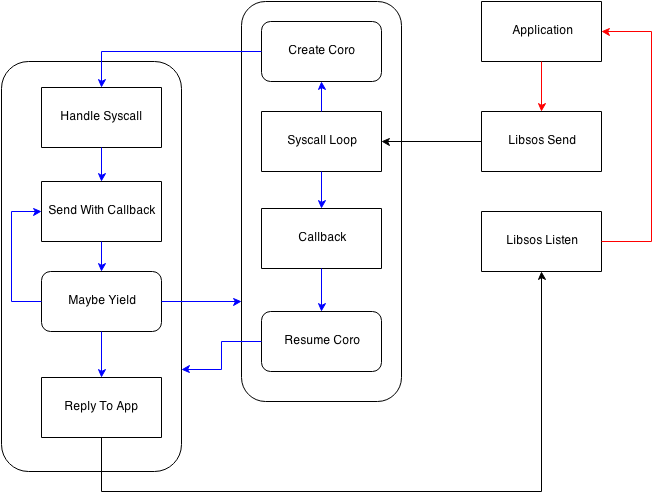
\includegraphics[scale=0.6]{System_Calls_Type2}
\caption{System Calls Operation}
\end{figure}

Stepping through;
\begin{enumerate}
\item Application does a system call
\item Libsos sends relevant information to SOS via IPC
\item SOS receives the message and determines the PID of the caller via its badge.
\item SOS then creates and executes a new coroutine assigned to the caller process.
\item If the system call involves being able to receive callbacks before continuing (eg. reading from nfs), we yield back to the main syscall loop. This way we avoid blocking the kernel.
\item When the callback comes through, we resume back to the point we left off in the handle syscall relating the PID of the original caller.
\item When no more operations need to be done, and the last call back comes through, we reply to the application
\item Libsos, depending on the system call, retrieve information received and return back to the main application.
\end{enumerate}

\clearpage
\section{File System}
\subsection{Interface}
Handle syscall functions;
\begin{itemize}
\item \textbf{void} syscall\_sys\_create(\textbf{pid\_t} mypid)\\
Sends NFS request to create a file with Read/Write permissions and yields to main.
\item \textbf{void} syscall\_sys\_open(\textbf{pid\_t} mypid)\\
Calls nfs\_lookup with path and yields to main.
\item \textbf{void} syscall\_sys\_close(\textbf{pid\_t} mypid)\\
Removes the file descriptor from the file table and yields to main.
\item \textbf{void} sys\_read\_routine(\textbf{struct read\_write\_data} *data)\\
Sends NFS requests one at a time and yields back to main. When this resumes, it repeats the process until no more reads are needed.
\item \textbf{void} syscall\_sys\_read(\textbf{pid\_t} mypid)\\
Gets information from message registers and checks permissions with file descriptor table. If the permissions for the file is write only, fail and reply back to caller. Otherwise, call sys\_read\_routine.
\item \textbf{void} sys\_write\_routine(\textbf{struct read\_write\_data} *data)\\
Sends NFS requests up to MAX\_IN\_FLIGHT (currently 4), then yields to the main syscall loop. When this next resumes, it will repeat the process until it has no more to send.
\item \textbf{void} syscall\_sys\_write(\textbf{pid\_t} mypid)\\
Gets information from message registers and checks permissions with the file descriptor table. If the permissions for the file is read only, fail and reply back to the caller. Otherwise, call sys\_write\_routine.
\item \textbf{void} syscall\_sys\_getdirent(\textbf{pid\_t} mypid)\\
Sets up tokens, calls nfs\_readdir and yields back to main.
\item \textbf{void} syscall\_sys\_stat(\textbf{pid\_t} mypid)\\
Calls nfs\_lookup with the path and yields back to main.
\end{itemize}
Callbacks;
\begin{itemize}
\item \textbf{void} nfs\_lookup\_reply(\textbf{uintptr\_t} token, \textbf{enum nfs\_stat} status, \textbf{fhandle\_t} *fh, \textbf{fattr\_t} *fattr)\\
Callback function for the sys\_stat syscall. Replies to original caller.
\item \textbf{void} nfs\_create\_reply(\textbf{uintptr\_t} token, \textbf{enum nfs\_stat} status, \textbf{fhandle\_t} *fh, \textbf{fattr\_t} *fattr)\\
Callback function for the sys\_create syscall. Replies to original caller.
\item \textbf{void} nfs\_open\_reply(\textbf{uintptr\_t} token, \textbf{enum nfs\_stat} status, \textbf{fhandle\_t} *fh, \textbf{fattr\_t} *fattr)\\
Callback for the sys\_open syscall. Replies to original caller.
\item \textbf{void} nfs\_readdir\_reply(\textbf{uintptr\_t} token, \textbf{enum nfs\_stat} status, \textbf{int} num\_files, \textbf{char} *file\_names[], \textbf{nfscookie\_t} nfscookie)\\
Callback for the sys\_getdirent syscall. Replies to original caller.
\item \textbf{void} nfs\_read\_reply(\textbf{uintptr\_t} token, \textbf{enum nfs\_stat} status, \textbf{fattr\_t} *fattr, \textbf{int} count, \textbf{void} *data)\\
Callback for the sys\_read syscall. If not the last callback (ie, there are still things left to be read), then resume the coroutine corresponding to the pid of the original caller. Otherwise, reply to the original caller.
\item \textbf{void} nfs\_write\_reply(\textbf{uintptr\_t} token, \textbf{enum nfs\_stat} status, \textbf{fattr\_t} *fattr, \textbf{int} count)\\
Callback for the sys\_write syscall. If not the last callback (ie, the entire string has not yet been written), then resume the coroutine corresponding to the pid of the original caller. Otherwise, reply to the original caller.
\end{itemize}
\subsection{Operation}
Here is a diagram of the write operation.
\begin{figure}[htbp]
\centering
%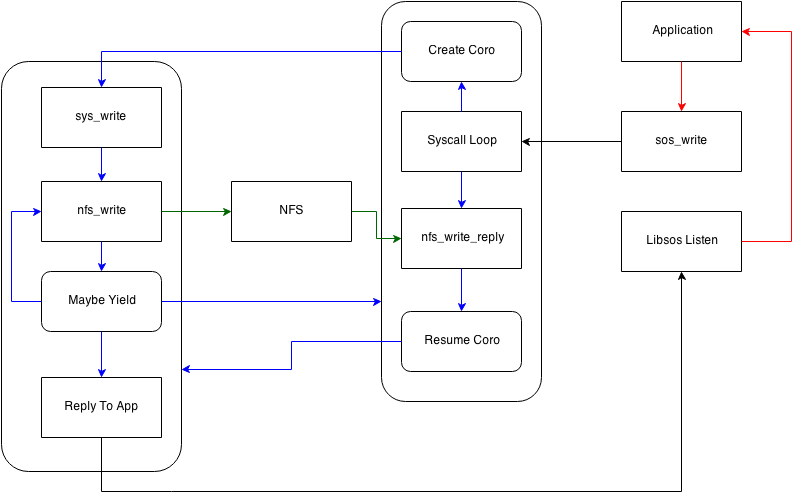
\includegraphics[scale=0.6]{SYS_WRITE}
\caption{File System Write Operation}
\end{figure}
Stepping through;
\begin{enumerate}
\item Application does a system call, passing through the address of the data array it wants to write via IPC
\item SOS receives the message and determines the PID of the caller via its badge.
\item SOS then creates and executes a new coroutine assigned to the caller process.
\item SOS copies 1024 bytes of data at a time from the address given by the application (translated into sos virtual address), into a temporary write buffer. The nfs\_write is called and the pid along with other information is passed through the token. After we send the maximum amount of NFS packets inflight at a time, we yield.
\item When the last callback comes through, we resume back to handle syscall and repeat step 4.
\item When no more operations need to be done, and the last call back comes through, we reply to the application with the total number of bytes written.
\end{enumerate}

The read operation is similar, however instead of copying data from the application in handle syscall, we copy read data from events to the application.

\clearpage
\section{Demand Paging}
\subsection{Interface}
\begin{itemize}
\item \textbf{int} frame\_swap\_in(\textbf{int} file\_index, \textbf{seL4\_Word} sos\_vaddr)\\
Swap in the frame that is in the swap file at position pointed to by file index
\item \textbf{int} frame\_swap\_out(\textbf{seL4\_Word} *vaddr)\\
Swap out the given frame, appends to swap file
\item \textbf{void} swap\_file\_create(\textbf{void})\\
Creates the swap file on NFS
\item \textbf{void} swap\_write\_reply(\textbf{uintptr\_t} token, \textbf{enum nfs\_stat} status, \textbf{fattr\_t} *fattr, \textbf{int} count)\\
Callback function for swapping out
\item \textbf{void} swap\_read\_reply(\textbf{uintptr\_t} token, \textbf{enum nfs\_stat} status, \textbf{fattr\_t} *fattr, \textbf{int} count, \textbf{void} *data)\\
Callback function for swapping in
\item \textbf{void} swap\_create\_reply(\textbf{uintptr\_t} token, \textbf{enum nfs\_stat} status, \textbf{fhandle\_t} *fh, \textbf{fattr\_t} *fattr)\\
Callback function for creating the swap file
\end{itemize}
\subsection{Operation}
\begin{itemize}
\item When a frame is allocated via vm fault, it is added to the frame queue. This is
done by two variables in each frame which point to the next frame and previous
frame in the queue.

\item For swapping out, we use a stack of indexes, as the order in which they return
when freed is inconsequential. These indexes are stored in the page table entry
of pages that are swapped out. When a page is in file, it has a infile bit set. On vm\_faults this bit is checked first and the frame swapped in if in file.

\item Swapping means we needed a method of blocking, as the nfs operation must complete before we can continue on in the program (to keep memory safe).
We used coroutines to carry this out, which simply yield back to the main loop after an nfs call, and return to the function on the nfs callback.
\end{itemize}

\clearpage
\section{Processes}
\subsection{Interface}
\begin{itemize}
\item \textbf{uint32\_t} init\_procs(\textbf{void})\\
Resets proccess array to default
\item \textbf{pid\_t} create\_process(\textbf{char} *app\_name, \textbf{uint32\_t} priority, \textbf{seL4\_CPtr} fault\_ep)\\
Finds the elf file given be "app\_name" that is contained within the cpio archive and creates a new process using that elf file.
\item \textbf{uint32\_t} destroy\_process(\textbf{pid\_t} pid)\\
Given a PID, destroys its address space, file descriptor table and frees any caps. If there were processes waiting for the process to be killed to finish, then resume them.
\item \textbf{uint32\_t} wait\_for\_process(\textbf{pid\_t} mypid, \textbf{pid\_t} pid, \textbf{seL4\_CPtr} my\_reply\_cap)\\
Adds mypid to target pid's waiting list, which will resume mypid when pid is destroyed. If target pid is -1, then add mypid to the global wait list, which will resume mypid when any process is destroyed.
\item \textbf{struct addrspace} *get\_proc\_addr\_space(\textbf{pid\_t} pid)\\
Gets the pointer to the address space of pid.
\item \textbf{fdtable} get\_proc\_fd\_table(\textbf{pid\_t} pid)\\
Gets the file descriptor table of pid
\item \textbf{cspace\_t} *get\_proc\_cspace(\textbf{pid\_t} pid)\\
Gets the cspace of this process.
\item \textbf{coro} get\_proc\_coro(\textbf{pid\_t} pid)\\
Gets the coroutine of this process.
\item \textbf{seL4\_CPtr} get\_proc\_ipc\_reply\_cap(\textbf{pid\_t} pid)\\
Gets the reply cap of the process.
\item \textbf{uint32\_t} get\_proc\_stime(\textbf{pid\_t} pid)\\
Gets the time since boot that the process was started at.
\item \textbf{uint32\_t} get\_proc\_size(\textbf{pid\_t} pid)\\
Gets the size of the process in pages.
\item \textbf{char} * get\_proc\_name(\textbf{pid\_t} pid)\\
Gets the name of the process.
\item \textbf{char} get\_proc\_taken(\textbf{pid\_t} pid)\\
Returns whether or not the pid number is in use.
\item \textbf{coro} create\_coro(\textbf{pid\_t} pid, \textbf{void} *fun(\textbf{void} *arg))\\
Creates a new coroutine unique to the process.
\item \textbf{void} set\_proc\_ipc\_reply\_cap(\textbf{pid\_t} pid, \textbf{seL4\_CPtr} cap)\\
Sets the reply cap of the process.
\end{itemize}
\subsection{Structure}
The process struct;
\begin{itemize}
\item \textbf{seL4\_Word} tcb\_addr\\
TCB cap, stored for destroy purpose
\item \textbf{seL4\_TCB} tcb\_cap\\
TCB cap, stored for destroy purpose
\item \textbf{struct addrspace} *as\\
The address space for this process, including the page table and region list
\item \textbf{fdtable} fd\_table\\
File descriptor table for this process, used for file systems
\item \textbf{seL4\_Word} ipc\_buffer\_addr\\
IPC buffer cap, stored for destroy purpose
\item \textbf{seL4\_CPtr} ipc\_buffer\_cap\\
IPC buffer cap, stored for destroy purpose
\item \textbf{cspace\_t} *croot\\
The croot for this process
\item \textbf{seL4\_CPtr} ipc\_reply\_cap\\
The reply cap for this process
\item \textbf{pid\_t} wait\_list[MAX\_PROC]\\
List of processes waiting for this process to finish
\item \textbf{uint32\_t} num\_waits\\
Num of other processes waiting on this process to finish
\item \textbf{coro} proc\_coro\\
The process coroutine, used for handle syscalls while not blocking kernel
\item \textbf{uint32\_t} stime\\
Time after boot at which the process was started
\item \textbf{uint32\_t} size\\
Size of the application in pages
\item \textbf{char} name[N\_NANME]\\
Name of the application, currently maximum 32 characters
\item \textbf{uint32\_t} name\_length\\
Length of the application name
\item \textbf{char} taken\\
When taken is not 0 then pid is in use.
\end{itemize}

There is an array "proc\_array" that contains a bunch of these structures and the index represents the PID.
\subsection{Operation}
\begin{itemize}
\item The processes infrastructure is initialized in main before the first process is created. This ensures that all the processes in the process list is set to their default values. 

\item When create is called, it assigns the process the lowest available pid number and a badge is created based on a offset of the pid number. An address space including page table is created for this process and regions for heap and stack are defined. Then its cspace is defined and an IPC buffer is created, the fault endpoint is minted to the process and a TCB object is created. Now, we either load the elf file from nfs or if it is the first process, load from cpio. Then we map in the stack, ipc buffer and start the process.

\item When destroy is called we reply to all processes waiting on the current process and also all processes in the global wait list. Then we destroy the file descriptor table, unmap the ipc buffer cap. The free the ipc buffer using ut\_free. Then we free the ipc\_reply\_cap, and destroy the cspace. Now we free the TCB object and destroy the address space. Finally, make the pid available for a new process again.
\end{itemize}
\clearpage
\section{ELF Loading}
\subsection{Interface}
\begin{itemize}
\item \textbf{int} elf\_load\_from\_nfs(\textbf{struct addrspace} * as, \textbf{const char} *name, \textbf{pid\_t} pid)\\
Loads elf file given by "name" into the address space of process given by "pid".
\item \textbf{void} elf\_lookup\_reply(\textbf{uintptr\_t} token, \textbf{enum nfs\_stat} status, \textbf{fhandle\_t} *fh, \textbf{fattr\_t} *fattr)\\
Callback for nfs\_lookup
\item \textbf{void} elf\_read\_reply(\textbf{uintptr\_t} token, \textbf{enum nfs\_stat} status, \textbf{fattr\_t} *fattr, \textbf{int} count, \textbf{void} *data)\\
Callback for nfs\_read 
\item \textbf{void} elf\_segment\_read\_reply(\textbf{uintptr\_t} token, \textbf{enum nfs\_stat} status, \textbf{fattr\_t} *fattr, \textbf{int} count, \textbf{void} *data)\\
Callback for nfs\_read, used in load\_segment\_into\_vspace2
\item \textbf{static int} load\_segment\_into\_vspace2(\textbf{struct elf\_nfs\_data} *nfs\_data, \textbf{char} *src, \textbf{unsigned long} segment\_size, \textbf{unsigned long} file\_size, \textbf{unsigned long} dst, \textbf{unsigned long} permissions)\\
Loads the elf file obtained from nfs to address space
\item \textbf{int} elf\_load2(\textbf{struct elf\_nfs\_data} *nfs\_data, \textbf{char} *elf\_file)\\
Loads the elf file obtained from nfs to address space, calls load\_segment\_into\_vspace2

\end{itemize}
\subsection{Operation}
\begin{itemize}
\item Elf loading from the NFS server was done by initially reading in the elf file header. From here, the points in the file which had to be read were done so by nfs, and then copied into the corresponding frame allocated. This was done one packet at a time. Due to the nfs operation we had to use coroutines, as with demand paging.
\end{itemize}

\section{Old File System Benchmarks}
We benchmarked the filesystem for milestone 5 which had a different implementation than what we currently have (The old system was difficult to adapt to demand paging, the new system is slower with writes at about 1Mb/s, because we are only sending 4 packets at a time with 1024 bytes per packet).

All benchmarking was done without the ethernet dongle and our mean speed at 30 packets in flight, 1284 bytes per packet is 4Mb/s for write and almost 17Mb/s for read. I had to artificially slow down reading, any more and we would get spurious interrupts slowing things down again.

\begin{figure}[htbp]
\centering
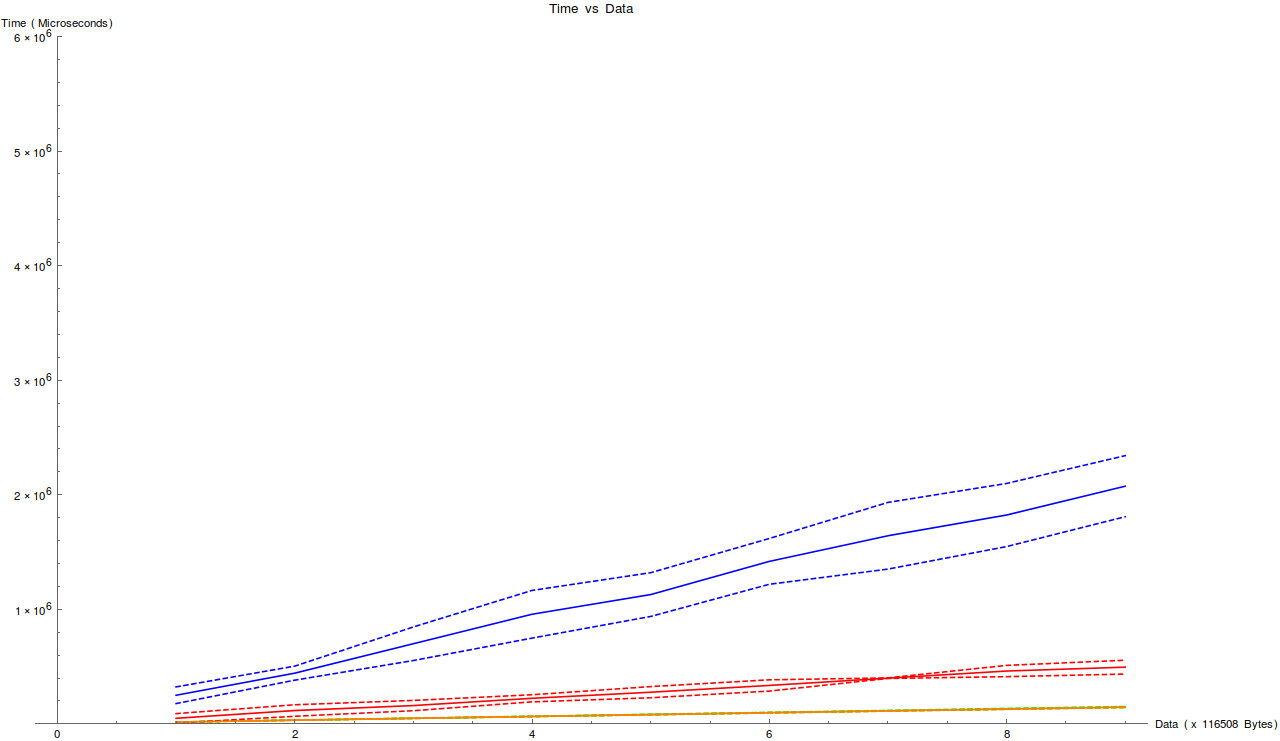
\includegraphics[scale=0.35]{benchmark_true_30_3}
\caption{The Blue line is write, and the red line is read.
The green and orange lines are overhead for write and read respectively.}
\end{figure}
\begin{figure}[htbp]
\centering
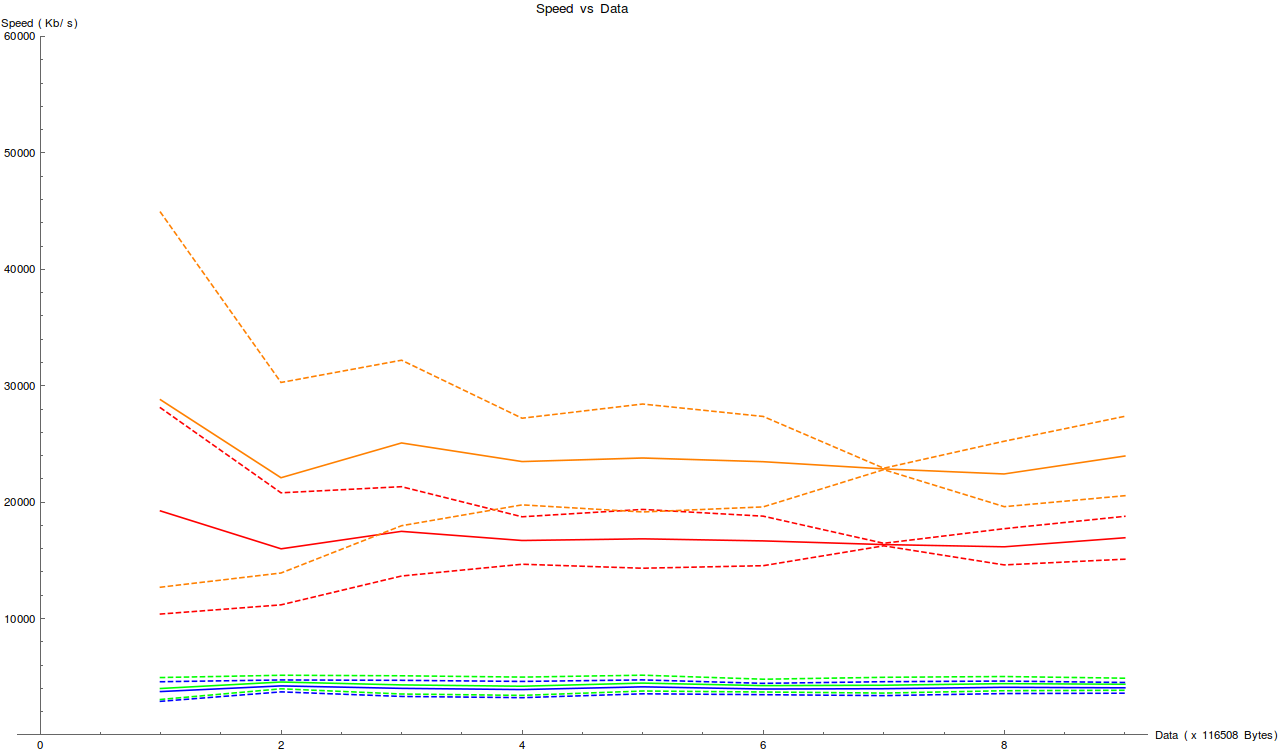
\includegraphics[scale=0.35]{benchmark_true_speed_30_3}
\caption{The Blue line is write, and the red line is read.
The green and orange lines are "ideal" speeds (minus overhead) for write and read respectively.}
\end{figure}
\begin{figure}[htbp]
\centering
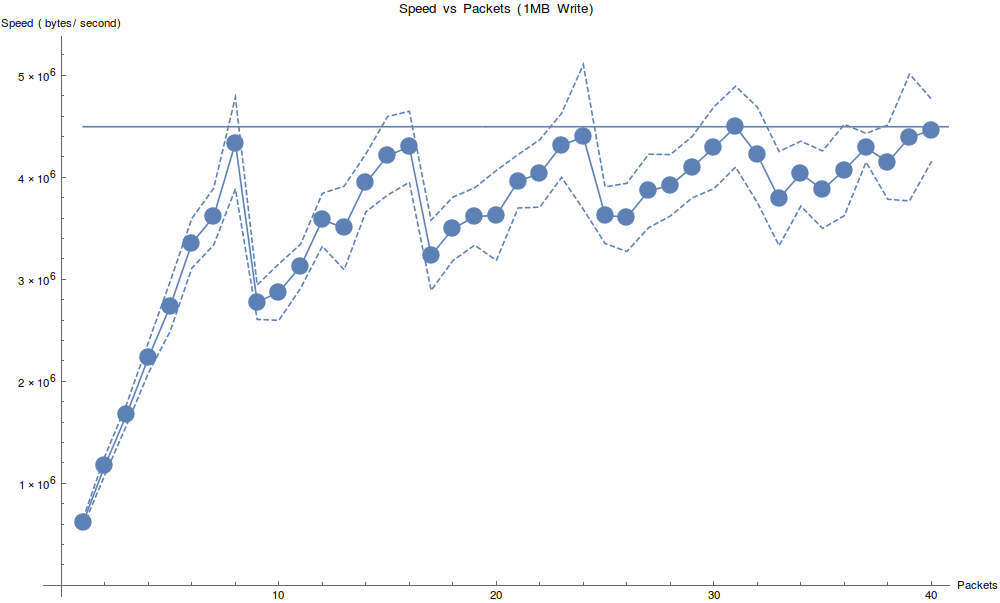
\includegraphics[scale=0.45]{benchmark_inflight}
\caption{The is a graph of speed of writing a 1MB file vs maximum number of packets inflight, interestingly, it follows a zig zag pattern, it seems that the optimal is 30 packets in flight}
\end{figure}

\end{document}
